\section{Experiments}
\label{sec:exp}
In this section, we evaluate how well Chameleon and its variants preserve a graph's structural statistics by comparing its anonymized \emph{uncertain} graphs against the original one in terms of graph metrics. Strong structural similarity (small error) in these results would establish the utility of these anonymized graphs in real research analysis and experiments. 

\subsection{Evaluation Metrics}
Besides reliability, our evaluation includes three classes of graph metrics. 
One group includes degree-based metrics such as Average Node Degree, Degree Distribution, Maximal Degree. These are basic topological metrics capture how degree distributed among nodes and how nodes with particular degree connect among others. The second group includes node separation metrics such as Average Distance, Graph Diameter. They are used to quantifying the inter-connectivity of the graph. The third group metrics include Clustering Coefficient which measures how close neighbors of a node are to forming cliques.

\textbf{Computation}~~Since there does not exist the closed formula for graph metrics expect Average Node Degree, the results are approximated by Monte Carlo sampling. Specifically, we create a number of random instances of an uncertain graph, and we compute the expected value of each metric using the average of the sampled graphs. Here, we use 1,000 samples since it has been shown that $1000$ usually suffices to achieve accuracy converge~\cite{Potamias_K_2010,Jin_Distance_2011}. In particular, we use Approximate Neighborhood Function (ANF) \cite{Boldi_Rosa_Vigna_2011}, to approximate shortest path-based statistics. For each metric, we report the ratio of absolute difference against the original one. 

\textbf{Parameter Setting}~~We generate anonymized \emph{uncertain} graphs for four obfusction levels, $k \in [100,300]$ and compare the graph metrics of the resulting \emph{uncertain} graphs against those original graphs. We limit ourselves to four obfusction levels for following reasons. 
First, we aim to explore the case the desired privacy level requires a small amount of noise ($k=100$). This way, we can quantify the utility loss difference introduced by Chameleon against Rep-An method. Second, it naturally requires a high level of noise to provide strong levels of privacy guarantees. We want to explore the sensitivity of different variants. Unfortunately, very large values of $k$ require large noise, thus producing anonymized graphs that are extremely different from the original ($k=300$). 


\subsection{Results}
\begin{figure*}[!tb]
    \centering
    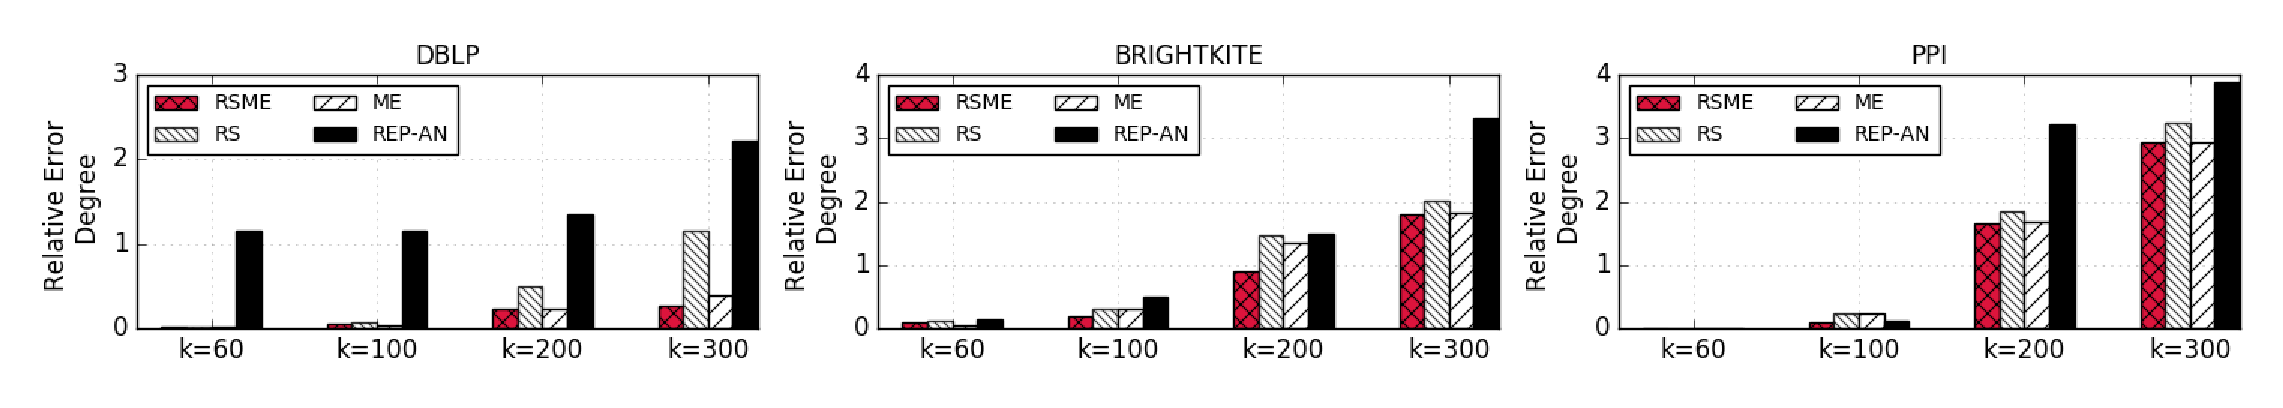
\includegraphics[width=\linewidth]{exp/ex_degree.eps}
    \caption{Comparison of anonymization methods in terms of their ability of preserving Average Node Degree.}
    \label{fig:ex_degree}
\end{figure*}


\begin{figure*}[!tb]
    \centering
    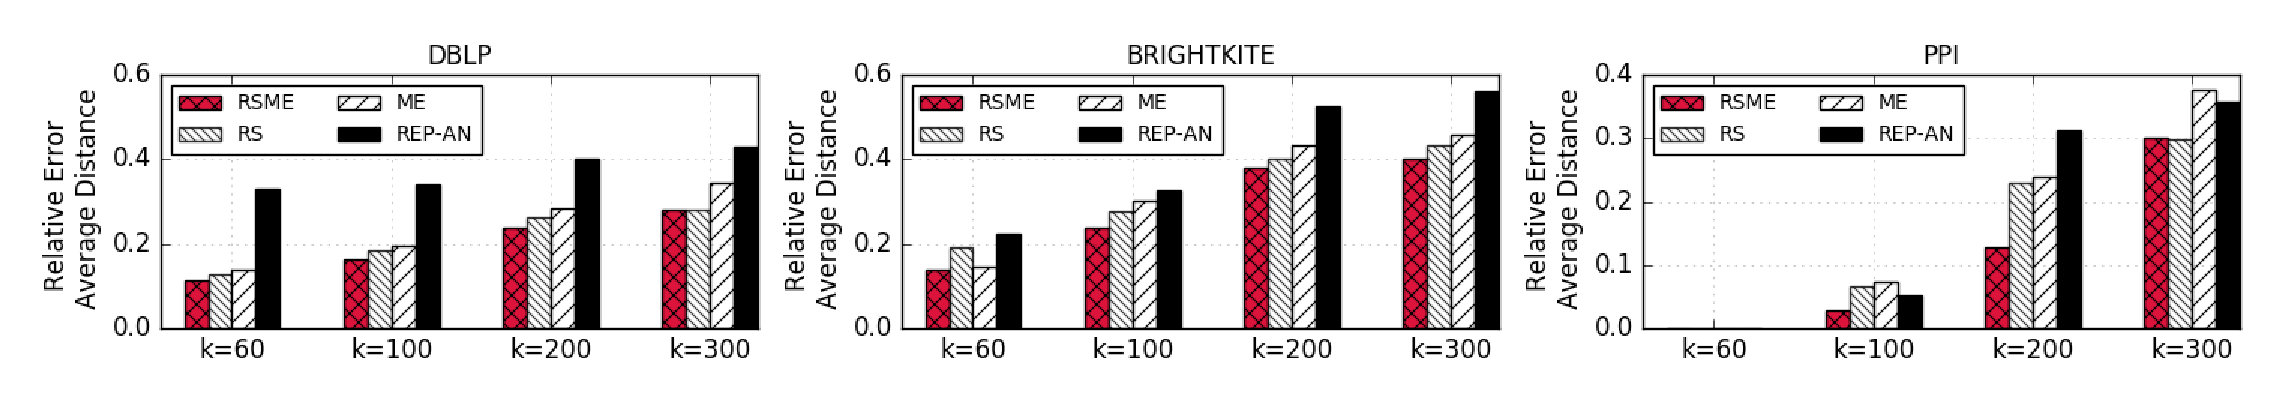
\includegraphics[width=\linewidth]{exp/ex_apd.eps}
    \caption{Comparison of anonymization methods in terms of their ability of preserving Average Distance.}
    \label{fig:ex_apd}
\end{figure*}

\begin{figure*}[!tb]
    \centering
    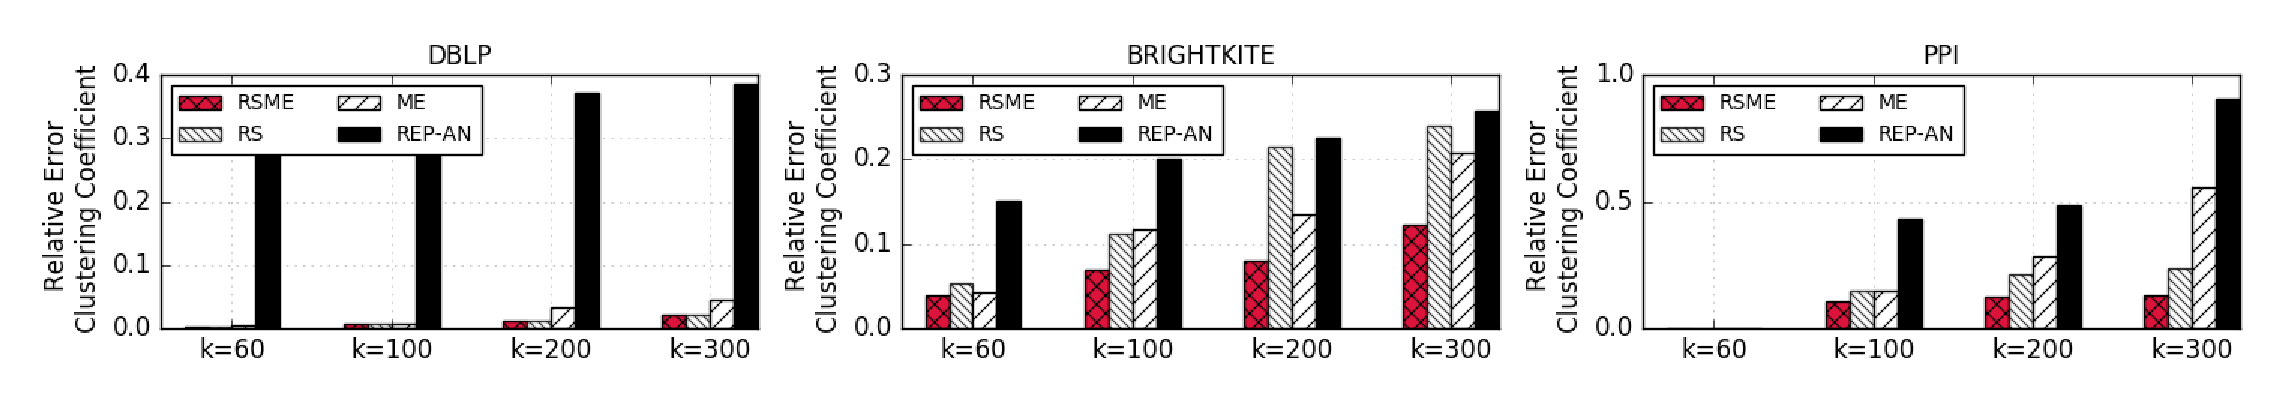
\includegraphics[width=\linewidth]{exp/ex_cc.eps}
    \caption{Comparison of anonymization methods in terms of their ability of preserving Clustering Coefficent.}
    \label{fig:ex_cc}
\end{figure*}

\textbf{Degree-based Metrics.}~~For brevity, we report results for  Average Node Degree. 
% \emph{Average Node Degree.}~~
Figure~\ref{fig:ex_degree} compares the average node degrees. For each of the DBLP, BRIGHTKITE and PPI graphs, the average node degrees of Chameleon ($k=100$) output graphs are very close the ones of the original graphs. When we increase the strength of the privacy guarantees, i.e., larger $k$ values of $200$ and $300$, the error of average degree progressively increases. For example, DBLP graph shows a small deviation even for $k=300$. The worst-case average degree deviation is still within 15\% of the original. 

On the other hand, BRIGHTKITE and PPI show slightly different behaviors. For large $k$ values, i.e., $k=200$ and $k=300$, the largest error is over 300\% from the original values. We attribute them to the existence of heavy-tailed degree distribution in these two graphs which requires more perturbation. 


\textbf{Node Separation Metrics.}~~For brevity, we report only the Average Distance as a representative of the node separation metrics. Figure~\ref{fig:ex_apd} shows the Average Distance (AD) values computed on DBLP, BRIGHTKITE, and PPI graphs compared to the AD values on their anonymized graphs. In this case, all of Chameleon output graphs do a good job of preserving the average distance of the original graphs. 



\textbf{Clustering Coefficent}


\textbf{Summary.}~~Our experimental assessment on real-world datasets confirms the initial and driving intuition: the {\SysNameNS} approach which explicitly incorporates edge uncertainty and the possible world semantic in the anonymization process outperforms the baseline \textsf{Rep-An} approach significantly regarding the uncertain graph utility preservation. The {\SysNameNS} introduces limited impact as a result of adding noise to guarantee privacy. And, the efficiency of the {\SysNameNS} approach is similar to the one of the \textsf{Rep-An} approach. 

Another message is: by using fine-grained and uncertainty-aware perturbation strategies such as reliability sensitive edge selection (RS) and max entropy based edge prob alteration (ME), one can achieve the same desired level of obfuscation with the smaller change on the uncertain graph thus maintaining higher data utility. 




